%
%  MP_talk.tex
%
%  Created by Steven Harms (HOME) on 2011-07-26.
%  Copyright (c) 2011 Steven G. Harms. All rights reserved.
%
\documentclass[slidestop,compress,mathserif]{beamer}
% \documentclass[slidestop,compress,mathserif, slidesonly]{beamer}
% Toggle between 'notes' and no notes to display or undisplay notes pages

% \usepackage[bars]{beamerthemetree}
\usetheme{PaloAlto}
\usecolortheme{seahorse}

% Use utf-8 encoding for foreign characters
\usepackage[utf8]{inputenc}

% Surround parts of graphics with box
\usepackage{boxedminipage}

% Package for including code in the document
\usepackage{listings}

% This is now the recommended way for checking for PDFLaTeX:
\usepackage{ifpdf}

% Support for handouts
\usepackage{pgfpages}
% \pgfpagesuselayout{4 on 1}[a4paper,border shrink=5mm]

\ifx\pdftexversion\undefined
\usepackage[dvips]{graphicx}
\else
\usepackage{graphicx}
\DeclareGraphicsRule{*}{mps}{*}{}
\fi
\title{Practical Metaprogramming:  Modeling Thought}
\author{ Steven G. Harms }

\date{2011-08-12}

\begin{document}

\ifpdf
\DeclareGraphicsExtensions{.pdf, .jpg, .tif}
\else
\DeclareGraphicsExtensions{.eps, .jpg}
\fi


\section{Introduction} % (fold)
\label{sec:introduction}
\begin{frame}
	\maketitle
\end{frame}

\subsection{Administration}
\begin{frame}
	\frametitle{Contact Me!}
	\begin{center}
		Steven G. Harms \\
		\vskip 1.25cm	
		Physically:  San Francisco, CA\\
		Email:  \texttt{lsrcv@sgharms.oib.com} \\
		Twitter / GitHub:  \texttt{sgharms} \\
		G+
	\end{center}
\end{frame}

\note{
Good afternoon, I want to welcome you all to the first day of Lone Star Ruby
Conference V. 
}

\begin{frame}
	\frametitle{Austin}
	\begin{center}
		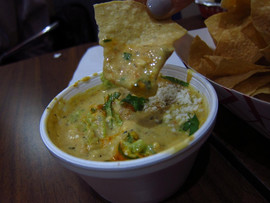
\includegraphics[scale=0.75]{img/queso.JPG}	
		\vskip 0.5cm
		\emph{Austin has many charms.  This is from Torchy's}
	\end{center}
\end{frame}
\note{
It's great to be back here in Austin. I've lived here for over
eight years off and on and love this town, its vibrant Ruby community, and
creativity with turning cheese into a soup that you put chips in. If you don't
know what I'm talking about, talk to me later and we'll get you set up
properly.
}


\subsection{Overview}

\begin{frame}
	\frametitle{What We'll Cover}
	\begin{center}
		Practical Metaprogramming:  ``Modeling Thought''
	\end{center}
\end{frame}
\note
{
\tiny
Today I would like to talk to you about \emph{Practical Metaprogramming}.
After one gets one's basic bearings in Ruby, it's not too long before one is
exposed to the magical world of Metaprogramming. In fact, sometimes it is the
reason people take up Ruby in the first place.
\\
Can I get a quick show of hands? Who was introduced to Ruby as a side effect
of ``Hey isn't it neat that Ruby can do this?'' How many of you have no idea
what I'm talking about when I say ``metaprogramming?''
\\
Regrettably, most of the time MP is introduced as a gimmick. Or, after it's
introduced, you may have a ``helpful'' colleage or friend who insists that
using MP is dangerous or something similar. I believe that if one is in that
spot, that's precisely where ``Practical Metaprogramming'' comes in. It can
help you dispel FUD, feel confident in metaprogramming, and realize why you
can't hide from it.
\\
As a tool as you undertake this transition as a Rubyist, I provide a concept
called ``Modeling thought.'' This refers to a technique or a dispotition which
is designed to help intermediate metaprogrammers evaluate whether an MP-based
solution is the right solution for them.  While not infallible, it's a good
rule of thumb.
\\
Let me take another quick poll: How many of you have never seen or heard about
Ruby's metaprogramming model? OK, well, I believe you will also be able to
benefit from this discussion as well and it may help you shape how you
approach learning the details of Metaprogramming.
\\
I also want to level set with you all, especially among those new to MP, I
will not have the ability to cover all the MP code blocks within the time we
have today. I will cover \emph{some} of the most important spells, but an
exhaustive tour is outside of our scope for the day.
\normalsize
}

\begin{frame}
	\frametitle{Goals}
	\begin{enumerate}
		\item Consider how we learn MP in the Ruby community
		\item Demonstrate that MP is a common style of thinking, and should be a common style of coding
		\item Provide a rubric for when to reach for the MP-hammer
		\item Give you the confidence to use MP \textbf{boldly}
		\item Provide a real-world example
	\end{enumerate}
\end{frame}
\note{
That's the lay of the land for this talk. If you're thinking this talk might
not be for you, then you're welcome to hop over.
}

\begin{frame}
	\frametitle{Intermission}
	\begin{center}
		\texttt{INTERMISSION}
	\end{center}
\end{frame}

\begin{frame}
	\frametitle{Socially Awkward Penguin}
	\begin{center}
		
\includegraphics[scale=0.3]{img/sap.png}			
	\end{center}	
\end{frame}
\note{
Whew, I'm glad we only lost those few. 
}

\begin{frame}
	\frametitle{End Slide if Everyone Leaves}
	\begin{center}
		
\includegraphics[scale=0.25]{img/forever_alone.png}
	\end{center}
\end{frame}


\section{Practical MP} % (fold)
\label{sub:practical_metaprogramming}

\section{Modeling Thought} % (fold)
\label{sec:modeling_thought}

\begin{frame}
	\begin{center}
		Practical Metaprogramming
	\end{center}
\end{frame}

\subsection{Early Exposure} % (fold)
\label{sub:early_exposure}

\begin{frame} 
	\frametitle{``Practical Metaprogramming:  First Contact''}
	
\includegraphics[scale=0.55]{img/first_contact.jpg} \\
	\emph{\ldots and is it to be called an ``eigenclass'' or a ``singleton class?''}
\end{frame} 
\note{
To understand practical metaprogramming I think it's helpful to imagine the
path of someone new to Ruby coming into first contact with the unique and
powerful metaprogramming capabilities of Ruby. In short to ask: ``How do we
start exploring MP in Ruby?''
}

\begin{frame} \frametitle{To Metaprogramming via Ruby}
	\texttt{attr\_*} \emph{Page 30}
	\vskip 0.5cm
	\begin{center}
		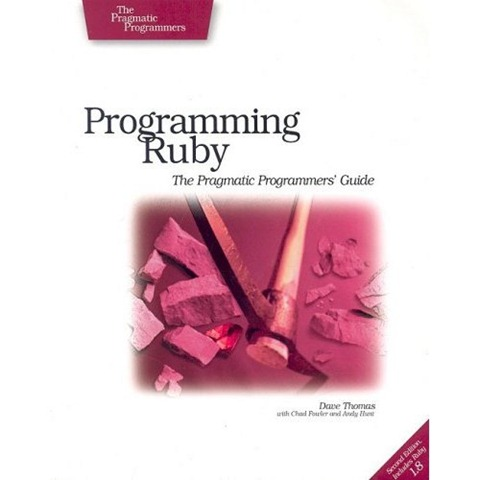
\includegraphics[scale=0.45]{img/ruby_pickaxe.jpg}	
	\end{center}
\end{frame} 
\note{For many Ruby developers, our first exposure to the world of
Metaprogramming starts around page thrity of the PickAxe book when we are
introduced to attr\_reader, attr\_writer, and attr\_accessor. 
}

\begin{frame}
	\frametitle{Dynamic Getter / Setter Generation}
	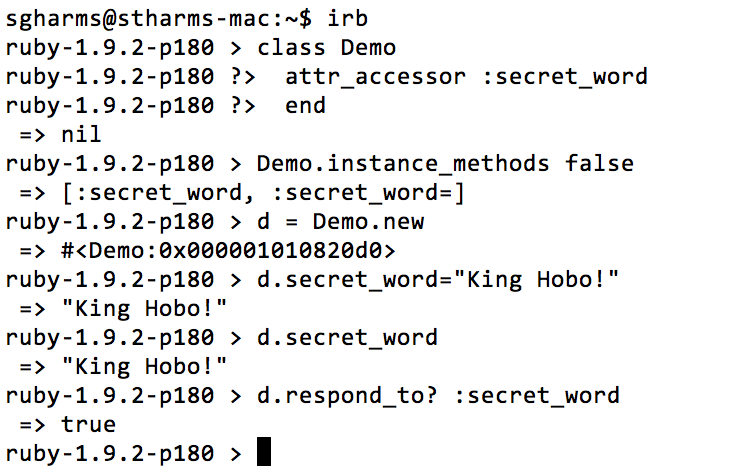
\includegraphics[scale=0.45]{img/attr_demo_1.png}	
\end{frame}

\begin{frame}
	\frametitle{Dynamic Getter / Setter Generation (2)}
	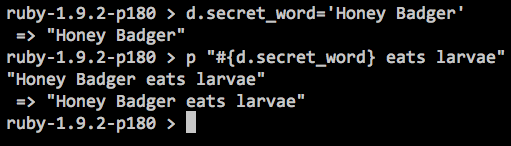
\includegraphics[scale=0.45]{img/attr_demo_2.png}	
\end{frame}

\begin{frame} \frametitle{To Metaprogramming via Rails}
	Rails (\texttt{order.discount=0.5}):  \emph{Page 28}
	\begin{center}
		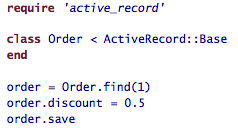
\includegraphics[scale=0.55]{img/awdwr_mp.png}	
	\end{center}
\end{frame}
\note{ Further, given that many people come to Ruby \emph{via} Rails, Rails
asks us to accept a great many things as ``magic'' as we get underway with it.
Rails first presents MP on page 28 in the context of how ActiveRecord maps
database fields to instance variables in its object-relational mapping. In
this case, having done nothing in the class \texttt{Order}, ActiveRecord does
the work and finds out from the database that the table schma has field
\texttt{discount} and that it should have getters and setters for it
fabricated -- not unlike what happened in the Ruby example.
}

\begin{frame}
	\frametitle{``Practical Metaprogramming''}
	\begin{itemize} 
		\item \texttt{attr\_*}:  \emph{Page 30}
		\item Rails (ORM):  \emph{Page 28}
	\end{itemize}
\end{frame}

\note{This is generally a suitable beginning and once we accept that we live
in a world laced with metaprogramming magic, we're generally content to simply
inhabit it. In this phase of our development, we don't know that
metaprogramming is going on, really. We accept these metaprogrammatic
behaviors as if they were core features of the language or the framework.

However, as we start to explore more about Metaprogramming, we start to move
to a place that, I contend, is generally \emph{impractical}.}

% subsection early_exposure (end)
\subsection{Intermediate Use} % (fold)
\label{sub:intermediate_use}

\begin{frame}
	\frametitle{Terminology}
	``Spells'' and their names derive from \underline{Metaprogramming Ruby} by Paolo ``Nusco'' Perrotta
	\vskip 0.5cm
	\begin{center}
		\underline{http://ducktypo.blogspot.com/2010/08/} \\
		\underline{metaprogramming-spell-book.html}
	\end{center}
\end{frame}
\note{
As a quick note, I thought I would add that I am going to be using the
terminology provided by Perrotta in his book. This is for two reasons. First
his names are good and I think that we, as a community, should find a common
lexicon for referring to these patterns. Furthermore, I want to recommend this
book for further exploration, so I would like to expose you to these
techniques in the language to which you will see them referred as.

There are about 30 of these ``spells,'' as Paolo calls them.
}

\begin{frame}
	\frametitle{``Slightly Impractical Metaprogramming:''  Open Classes}
	\begin{itemize}
		\item Open Classes
	\end{itemize}
		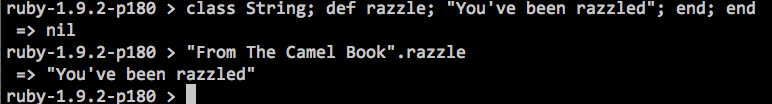
\includegraphics[scale=0.45,width=10cm,height=2cm]{img/open_class.png}	
\end{frame}
\note{It usually starts like this. You realize that you can add methods to an
existing class and add ``interesting'' features to classes. \emph{Describe
``Open Class''}.}


\begin{frame}
	\frametitle{``Slightly Impractical Metaprogramming:''  Kernel Method}
	\begin{itemize}
		\item Open Classes
		\item Kernel Method
	\end{itemize}
		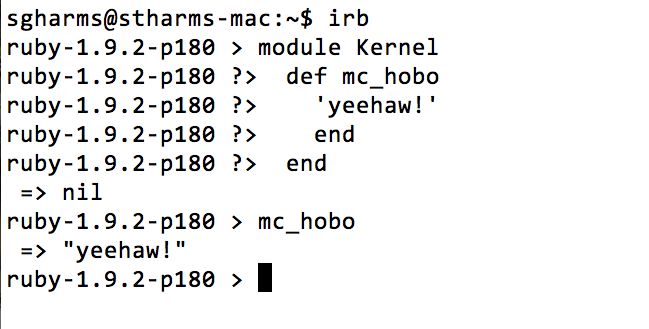
\includegraphics[scale=0.55]{img/kernel_method.png}	
\end{frame}
\note{
At this point we're starting to feel some power here. We now see that we can
create methods that behave as if they were core builtins to the language.
}

\begin{frame}
	\frametitle{``Slightly Impractical Metaprogramming:  Singleton Method''}
	\begin{itemize}
		\item Open Classes
		\item Kernel Method
		\item Singleton Method
	\end{itemize}
		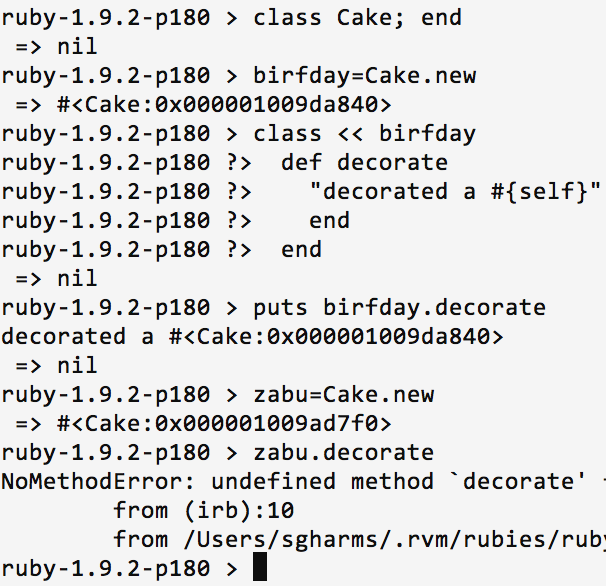
\includegraphics[scale=0.35]{img/singleton_method.png}
\end{frame}
\note{
This is undoubtedly the one that makes the pro-Java camp weep. In compiled
languages the definition of a class represents a static contract between the
developer and the compiler. A class is an expression of that contract. In
Ruby, a class is really a namespace expression. This is pretty cool stuff.
}

\subsection{Danger Zone} % (fold)
\label{sub:danger_zone}

\begin{frame}
		\frametitle{AWESOMENESS}
		\begin{center}
			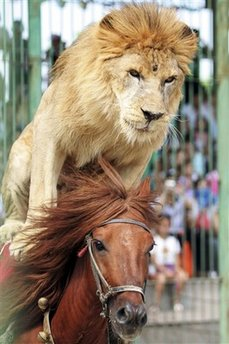
\includegraphics[scale=0.45]{img/lion_horse.jpg}
		\end{center}			
\end{frame}
\note{It might not be the most awesome thing ever, which is, of course, a lion riding a horse, but it's still pretty good.}

\begin{frame}
	\frametitle{Madness}
	This leads to the dangers of MP:
	\begin{itemize}
		\item Opaqueness
		\item Unpredictability
		\item Unsupportability
	\end{itemize}
	\begin{center}
			\emph{Abandon all hope ye who enter \ldots}
		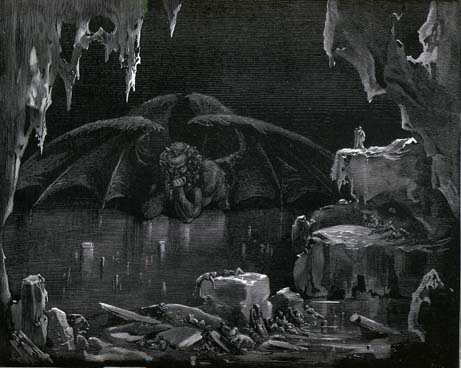
\includegraphics[scale=0.45]{img/dante.jpg}		
	\end{center}
\end{frame}
\note{Read aloud\ldots}

\begin{frame}
	\frametitle{Thesis:  F.U.D.}
		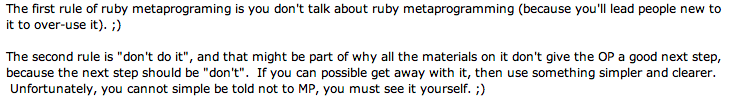
\includegraphics[width=0.98\textwidth, height=0.25\textheight]{img/tim_hates_mp.png}		
		\vskip 0.5cm
		\emph{--Tim Connor:  SF Ruby Mailing List}
\end{frame}
\note{
Read aloud\ldots. Note, I had a mail from Tim and his personal views aren't as
strong as this, but he's definitely urging caution over MP's over-use.
}

\begin{frame}
	\frametitle{Antithesis:  anti-F.U.D.}
	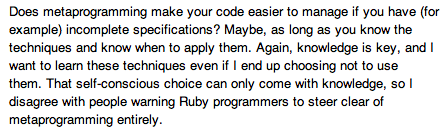
\includegraphics[width=0.98\textwidth, height=0.45\textheight]{img/paolo_anti_fud.png}		
	\vskip 0.5cm
	\emph{--Paolo Perrotta, author of Metaprogramming Ruby, in e-mail to Steven Harms}
\end{frame}

\subsection{Benefits} % (fold)
\label{sub:benefits}

\begin{frame}
	\frametitle{Synthesis:  You Need To Learn This:  Precedent}
	\begin{enumerate}
		\item Virtually all core libraries make use of MP
		\item Rails uses MP all over the place
	\end{enumerate}
	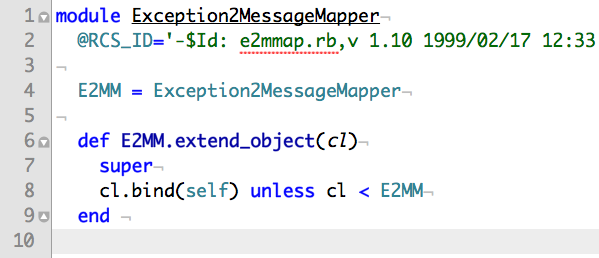
\includegraphics[scale=0.45, width=0.98\textwidth]{img/e2mmap.png}
\end{frame}

\begin{frame}
	\frametitle{Synthesis:  You Need To Learn This:  Your Future}
	\begin{enumerate}
		\item Save yourself a lot of typing
	\end{enumerate}
\end{frame}

\begin{frame}
	\frametitle{Synthesis:  You Need To Learn This:  Your Future}
	\begin{enumerate}
		\item Save yourself a lot of typing
		\item Reflect the interior world of your problem domain in your application code
	\end{enumerate}
\end{frame}

\begin{frame}
	\frametitle{Synthesis:  You Need To Learn This:  Your Future}
	\begin{enumerate}
		\item Save yourself a lot of typing
		\item Reflect the interior world of your problem domain in your application code
		\item Pleasant surprises
	\end{enumerate}
\end{frame}

\begin{frame}
	\frametitle{How Will I Know?}
	The key to knowing when to apply an MP solution is to turn the
\underline{benefits} just described into \underline{conditions}. Together they
form the basis of ``modeling thought.''
\end{frame}

\section{Modeling Thought} % (fold)
\label{sec:modeling_thought}

\begin{frame}
	\begin{center}
		Modeling Thought
	\end{center}
\end{frame}

\begin{frame}
	\frametitle{``Modeling Thought''}
	\large
	\centering{First Law \\ + \\ Second Law \\ = \\ }
	\vskip 0.5cm
	\begin{center}
		``Modeling Thought''
	\end{center}
	
	\normalsize
\end{frame}
\note{
``Modeling Thought'' is a conceptual rubric for evaluating when a solution
calls for a metaprogrammatic solution.

Let's transform those motivations just mentioned into some ``Laws'' and
``Corrolaries.''
}

\subsection{Laws} % (fold)
\label{sub:laws}

\begin{frame}
	\frametitle{First Law of Metaprogramming}
	\centering{\emph{	A metaprogrammatic solution is suitable when you need to provide
	unambiguous answers (return values) to ambiguously asked things (flexible /
	incomplete method calls)}
}\end{frame}
\note{
Now let me first be clear that I'm not saying these are laws as in
set-in-stone sense. Calling them ``guidelines'' seemed a bit weak,
``recommendations'' too. And I certainly don't expect that years hence there
will be schisms over proper adherence to ``Steven\'s laws of
metaprogramming.'' I'm trying to refer to a practical guideline with some heft
to it.
}

\begin{frame}
	\frametitle{First Law of Metaprogramming}
	\centering{\emph{	A metaprogrammatic solution is suitable when you need to provide
	unambiguous answers (return values) to ambiguously asked things (flexible /
	incomplete method calls)}
	\vskip 0.5cm
	\centering{\emph{e.g. Rails' ORM Calculation}}
}\end{frame}
\note{

Let's think about how Rails handles attribute definition. As a user of Rails
we can say things like ``Get my attributes.'' This is what the first law terms
an ``ambiguous request.'' Bear in mind, ``ambiguous'' here has no value
judgment, but is simply to say that the question could be, conceivably,
answered different ways on differing queries.

Nevertheless, for a given request, there is always a discrete, clear, singular
answer that is ``correct.'' Modeling for ambiguity and tolerance is something
that's harder to do in other languages, but that is a core principle of Ruby.
We'll talk more about that momentarily. Let's take a look at the second law.
}

\begin{frame}
	\frametitle{Second Law of Metaprogramming}
	\centering{\emph{ A metaprogrammatic solution is suitable when mechanical
recording of the the values is time inefficient when compared to learning the
generating heuristic}}
\end{frame}

\begin{frame}
	\frametitle{Second Law of Metaprogramming}
	\centering{\emph{ A metaprogrammatic solution is suitable when mechanical
recording of the the values is time inefficient when compared to learning the
generating heuristic}}
	\vskip 0.5cm
	\centering{\emph{e.g. attr\_* methods}}
\end{frame}
\note{
I consider typing a lot to be a code smell. If I find that I'm writing
anything where each so-called unique case is only different from another case,
then I start to get worried that I'm doing something wrong.

This is generally a good instinct to have in the world of object orientation,
but certain other languages make typing a lot (or defining pre-processor
macros that are effectively doing a lot of typing for you) seem like the
natural order of things. As Rubyists, we should eschew this tendency.

An interesting tendency has emerged during my work with Ruby's MP model, and
that's this first corrolary:
}

\begin{frame}
	\frametitle{First Corrolary:}
	\begin{center}
		\emph{Any significant metaprogramming work undertaken to meet either of
    the laws will eventually look like it was undertaken for a reason in
    service to the opposite law}
	\end{center}
\end{frame}

\begin{frame}
	\frametitle{Fascinating Symmetries:  Metaprogramming and Thinking}
	Law I:  \textbf{Thinking} provides unambiguous answers to ambiguously asked things \\
	Law II: \textbf{Thinking} is the more efficient learning of generating heuristics opposed to rote recording of data \\
	\vskip 0.5cm
	Symmetry is the basis of ``Modeling Thought''
\end{frame}

\begin{frame}
	\frametitle{``Modeling Thought: Born That Way''}
	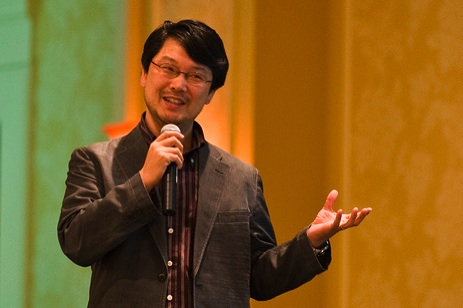
\includegraphics[scale=0.6]{img/matz.jpg}		
\end{frame}
\note{
And no language supports the ``modeling thought'' paradigm like Ruby. 
}

\begin{frame}
	\frametitle Stepwise Progress
	\begin{itemize}
		\item Matz' Design
		\item Paolo's ``Spells''
		\item A rule of thumb:  ``Modeling Thought''
	\end{itemize}
\end{frame}
\note{
Thanks to Matz' design, we can define 30-odd ``Spells'' enumerated by Perrotta
and put into his book. And now with a rule of thumb, we can start to achieve
consistency in how we use MP. As we are now more comfortable with our
expressions making use of metaprogramming, we can be bold and not worry about
the FUD, but can rather use MP \textbf{boldly}.
}

\subsection{LatinVerb} % (fold)
\label{sub:_modeling_thought_in_latinverb}

\begin{frame}
	\frametitle{LatinVerb}
	LatinVerb is a library for conjugating Latin verbs given their ``four principle parts''
\end{frame}

\begin{frame}
	\frametitle{Just Enough Latin}
	\vskip 0.5cm
	\begin{center}
		
\includegraphics[scale=0.45]{img/captain.jpg}
	\end{center}
	
	\vskip 0.5cm
	\begin{center}
		\emph{``Captain!  My Captain!''}
	\end{center}
	
\end{frame}

\begin{frame}
	\frametitle{Therefore\ldots}
	Given:  ``am\={o}, am\={a}re, am\={a}v\={\i}, amatum''
	\vskip 0.5cm
	Specific Vector: ``Active Voice / indicative mood / present tense/ first person / singular number'' 
	\vskip 0.5cm
	\begin{center}
		\emph{am\={o}}
	\end{center}
\end{frame}

\begin{frame}
	\frametitle{Unique Specification:  Stargate}
	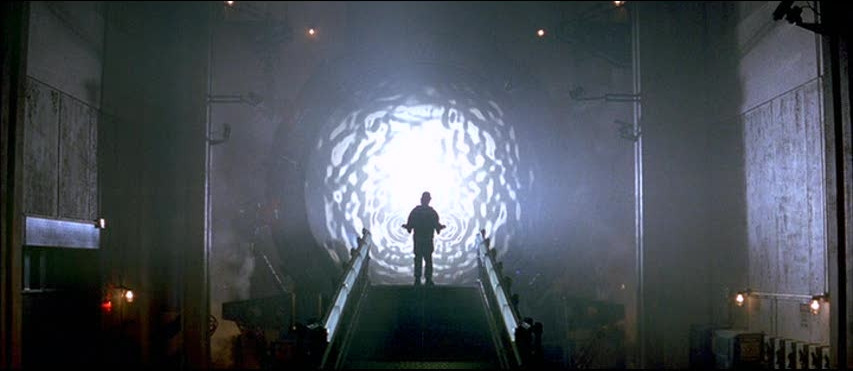
\includegraphics[scale=0.25]{img/stargate.jpg}
	\vskip 0.5cm
	\centering{6 Points in Space}
\end{frame}

\begin{frame}
	\frametitle{Unique Specification:  Latin}
	5 Aspects
	\begin{enumerate}
		\item voice
		\pause
		\item mood
		\pause
		\item tense
		\pause
		\item person
		\pause
		\item number
		\pause
	\end{enumerate}
	\vskip 0.5cm
	A unique coordinate is a \emph{vector}
\end{frame}

\begin{frame}
	\frametitle{Translating a Domain Problem to Ruby} 
	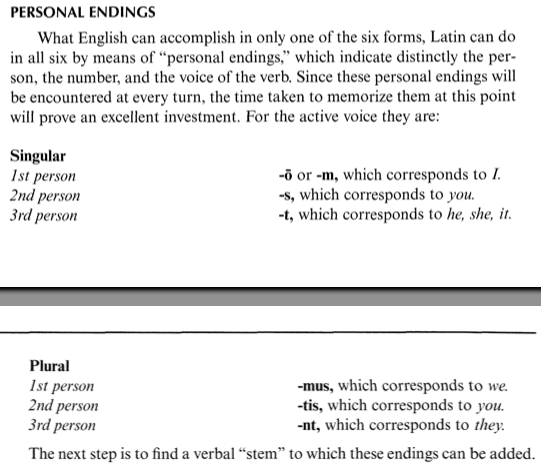
\includegraphics[scale=0.45]{img/conj_how_1.png}
\end{frame}

\begin{frame}
	\frametitle{Translating a Domain Problem to Ruby} 
	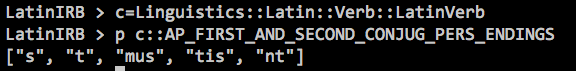
\includegraphics[scale=0.45]{img/conj_how_1b.png}
\end{frame}

\begin{frame}
	\frametitle{Translating a Domain Problem to Ruby} 
	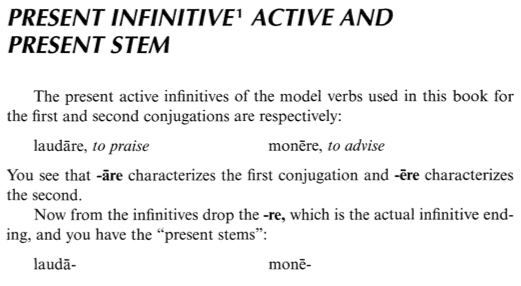
\includegraphics[scale=0.45]{img/conj_how_2.png}
\end{frame}

\begin{frame}
	\frametitle{Combine!}
	\emph{``Take an array of elements and tack them onto a base with the results
returned as an array. Why does that sound familiar?''}
	
\includegraphics[scale=0.45]{img/determined.png}
\end{frame}

\begin{frame}
	\frametitle{Translating a Domain Problem to Ruby} 
	\vskip 1.0cm
	\begin{center}
		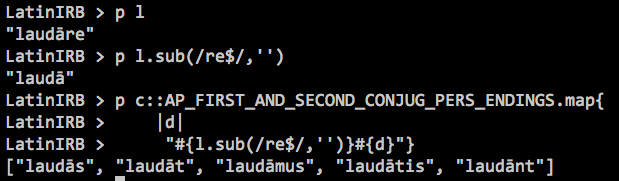
\includegraphics[scale=0.45]{img/conj_how_2b.png}	
	\end{center}
\end{frame}


\begin{frame}
	\frametitle{Translating a Domain Problem to Ruby} 
	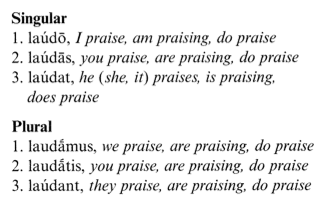
\includegraphics[scale=0.45]{img/conj_how_3.png}	
\end{frame}
\note{
I'm going to skip over some of the details here about the phongraphic rules
for shortening vowels and am going to provide the test case for correct
conjugation of this tense here:
}

\begin{frame}
	\frametitle{Translating a Domain Problem to Ruby} 
	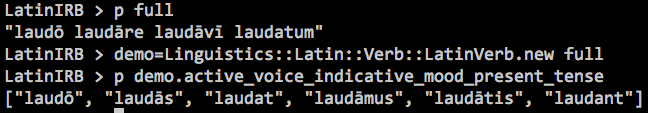
\includegraphics[scale=0.45]{img/conj_how_3b.png}	
\end{frame}
\note{
So what happens here? In LatinIRB (an IRB wrapper around LatinVerb that I
wrote). We specify the characterizing string. We use that string to create a
LatinVerb object and then we provide 3 of the 5 criteria required for
producing a single unique vector and as a result we acquire 6 answers. The
additional criteria would have to be added to get a specific unique value, as
we stated previously.

This is actually the way I memorized the materials for my Latin class. I just
remembered \texttt{map} operations.  This realization was very powerful, one 
of those ``a-ha'' moments that, while on the surface of it, was a very simple
concept, actually opened the gateways to other thoughts.
}

\begin{frame}
	\frametitle{Standard Domain Modeling}
	\begin{itemize}
		\item Generated results to save typing
		\item Implements a standardized heuristic (from \emph{Wheelock's Latin}) so that domain experts retain familiarity
	\end{itemize}
\end{frame}

\begin{frame}
	\frametitle Madness set in\ldots
	\vskip 1.0cm
	\emph{Could I scale this to \underline{all} Latin verbs?}
\end{frame}


\begin{frame}
	\frametitle{Painful Math}
	\begin{itemize}
		\item 6 results means 6 methods to be defined \emph{per tense}
		\pause
		\item \ldots $\times$ 6 tenses (present|imperfect|future|perfect|past-perfect|future-perfect)
		\pause
		\item \ldots $\times$ 2 voices (active|present)
		\pause
		\item \ldots \emph{and then there's another voice!}
		\pause
		\item Each regular Latin verb has $\approx$  160 unique vectors
		\pause
		\item There are 5 standard paradigms
		\pause
		\item \ldots and at least $1,000$ verbs
	\end{itemize}
\end{frame}

\begin{frame}
		\frametitle{Suck}
		\begin{itemize}
			\item Typing all of these several hundred(thousand?)-odd values in would definitely suck.
			\pause
			\item What if you had incomplete data?  4/5 of the vector specification?
		\end{itemize}
		\begin{center}
			\begin{tabular}{|c|c|c|}
				\hline
				  & Singular Number &  Plural Number\\
				\hline
				First Person  & laud\={o}  & laud\={a}mus\\
				Second Person & laud\={a}s & laudatis \\
				Thrid Person  & laudat     & laudant \\
				\hline
			\end{tabular}
		\end{center}
		\pause
		Law II says to MP our way out of the pain
\end{frame}


\begin{frame}
	\frametitle{ Use Metaprogramming}
	\begin{itemize}
		\item Could we make the result array \texttt{[laud\={o}, laud\={a}s, laudat laud\={a}mus, laudatis, laudant]} smarter?
		\pause
		\item Yes!
		\pause 
		\item Make that Array a class whose \texttt{method\_missing} resolves the last two aspects flexibly.
	\end{itemize}
\end{frame}


\subsection{Handling Ambiguity} % (fold)
\label{sub:methods}

\begin{frame}
	\frametitle{What It Looks Like}

	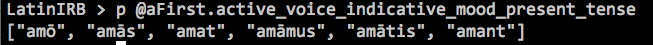
\includegraphics[scale=0.35]{img/flexibility_1.png}	
	\vskip 0.5cm
	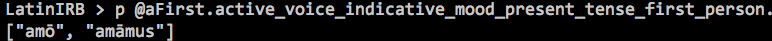
\includegraphics[scale=0.35]{img/flexibility_2.png}	
	\vskip 0.5cm
	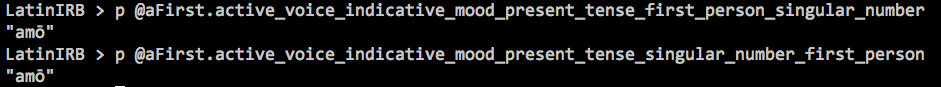
\includegraphics[scale=0.30]{img/flexibility_3.png}	
\end{frame}

\begin{frame}
	\frametitle{How To Do It:  Call to a Tense Returns a TenseBlock}
	\begin{center}
		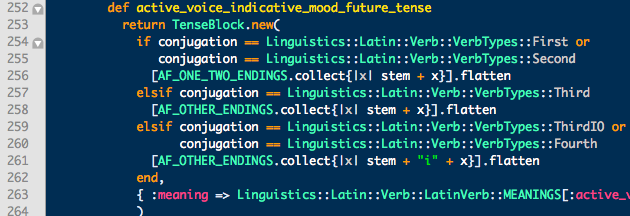
\includegraphics[scale=0.45]{img/tense_method_call.png}
	\end{center}
\end{frame}

\begin{frame}
	\frametitle{\underline{Ghost Method} in \texttt{TenseBlock}}
	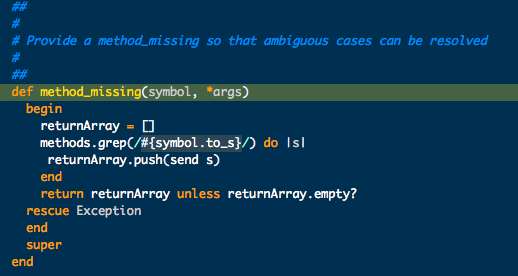
\includegraphics[scale=0.45]{img/tenseblock_mm.png}
\end{frame}


\begin{frame}
	\frametitle{Benefits}
	\begin{itemize}
		\item Saved many keystrokes by writing a class and \texttt{method\_missing} definition
		\pause
		\item Saved creating 6 additional methods per tense for vectors
		\pause
		\item Saved creating 5 additional ``aggregate methods'' per tense
		\pause
		\item Avoids C-style brain damage
		\pause
		\item More meaningful aggregate chunking
	\end{itemize}
\end{frame}
\note{I believe these first two benefits are obvious, so instead I'll focus on these other three.}

\begin{frame}
	\frametitle{C-ish Brain Damage:  Parameterization}	
 	\texttt{String calculate\_vector(VerbyType aV, String v, String m, String t, String p, String n)}
\end{frame}

\begin{frame}
	\frametitle{C-ish Brain Damage:  Parameterization}	
	\texttt{Object[] calculated\_values = \{aV, v, m, t, p, n\};} 
	\texttt{String calculate\_vector(calculated\_values)}; 
\end{frame}
\note
{A particular reason that I want to highlight this benefit is because C-style
parameterization is not how we think.
}

\begin{frame}
	\frametitle{Not How We Think}
	\begin{itemize}
		\item We \emph{do not} think like we are ordering from Subway.
		\pause
		\item NO:  \emph{``I'll have a sandwich:  bread is rustic Italian, meat is salami, cheese is provelone, veggies are an array of lettuce, tomato \ldots''}
		\pause
		\item YES:  \emph{``I'll have an Italian on rustic Italian with salami and provelone and from the veggie bin, lessee, lettuce and tomato\ldots''}
	\end{itemize}
	
\end{frame}
\note{This is probably something \emph{right} about the Objective-C language.}


\begin{frame}
	\frametitle{ ``Modeling Thought:''  Arbitrary Chunking}
	\begin{itemize}
		\item In Latin we talk about ``tenses'' as an aggregate of six vectors.  Let's use this as a ``chunk.''
		\pause
		\item We needn't be limited to Arrays, Hashes, Vectors, or other DS'
	\end{itemize}
\end{frame}

\begin{frame}
	\frametitle{MP Techniques Used}
	\begin{enumerate}
		\item Ghost Method:  Dont define a method (in \texttt{TenseBlock}) so that its \texttt{method\_missing} acts as \texttt{method\_called}
		\item Blank Slate:  A TenseBlock is a Blank Slate, effectively
		\item Dynamic Dispatch:  \texttt{self.send} in \texttt{TenseBlock}
	\end{enumerate}
\end{frame}

\begin{frame}
	\frametitle{The Corollary}
	\begin{itemize}
		\item 	We pursued ``less typing'' but wound up with ``respond to ambiguous calls with unambiguous data''
		\pause
		\item 	`Modeling Thought'' is full of these surprises
	\end{itemize}
\end{frame}

\begin{frame}
	\frametitle{Scale it Up!}
	\frametitle{method\_missing and method\_called}
	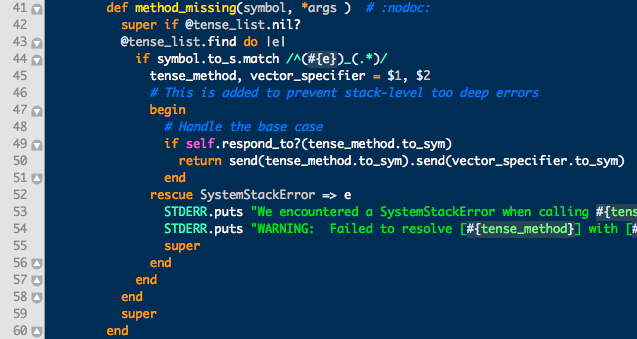
\includegraphics[scale=0.45]{img/lv_mm.png}	
\end{frame}

\begin{frame}
	\frametitle{Result}
	\begin{itemize}
		\item 24 methods
		\item One reponse class (\texttt{TenseBlock})
		\item Covered the thousands of methods predicted
		\item \ldots and provided the clustering methods as well as a surprising bonus
	\end{itemize}
\end{frame}

\begin{frame}
	\frametitle{This is the golden use of Metaprogramming}
\end{frame}


% ---- TO INCLUDE? ------
% \subsection{Domain-Specific Languages} % (fold)
% \label{sub:domain_specific_languages}
% \begin{frame}
% 	\frametitle{Placeholder}
% 	\ldots
% \end{frame}


%  Dynamic dispatch
% Dynamic method (definition)
% Extension by result from MP
% subsection domain_specific_languages (end)

% ---- TO INCLUDE? ------

% section modeling_thought (end)

\section{Supplementary} % (fold)
\label{sec:supplementary}

\begin{frame}
	\frametitle{Book}
	\underline{Metaprogramming Ruby} by Paolo Perrotta
\end{frame}

\begin{frame}
	\frametitle{List of Spells}
	\texttt{http://ducktypo.blogspot.com/2010/08/metaprogramming-spell-book.html}
\end{frame}

\begin{frame}
	\frametitle{Colophon}
	\LaTeX and the Beamer Slide Style
\end{frame}


% section supplementary (end)

\begin{frame}
	\frametitle{SpeakerRate}
	\centering{Help Me Get Better!}
	\vskip 1.25cm
	\centering{\texttt{http://speakerrate.com/talks/\\7831-practical-metaprogramming-modeling-thought}}
\end{frame}
\note{
At the conclusion of this presentation please take the time to help me out by
giving me some feedback about how things went. Please be honest, but
constructive. If the slides didn't advance the point, if you didn't like my
jokes. If the contrast or typeface are bad, please let me know.
}

\begin{frame}
	\frametitle{Contact Me!}
	\begin{center}
		Steven G. Harms \\
		\vskip 1.25cm	
		Physically:  San Francisco, CA\\
		Email:  \texttt{lsrcv@sgharms.oib.com} \\
		Twitter / GitHub:  \texttt{sgharms} \\
		G+
	\end{center}
\end{frame}

\end{document}

